\documentclass[9pt]{beamer}

\usetheme{Madrid}
\usecolortheme{default}
\setbeamertemplate{navigation symbols}{}

% Footer: title left, page number right
\setbeamertemplate{footline}
{
  \leavevmode%
  \hbox{%
  \begin{beamercolorbox}[wd=.5\paperwidth,ht=2.25ex,dp=1ex,center]{author in head/foot}%
    \usebeamerfont{author in head/foot}\insertshorttitle
  \end{beamercolorbox}%
  \begin{beamercolorbox}[wd=.5\paperwidth,ht=2.25ex,dp=1ex,right]{date in head/foot}%
    \usebeamerfont{date in head/foot}\insertshortdate{}\hspace*{2em}
    \insertframenumber{} / \inserttotalframenumber\hspace*{2ex}
  \end{beamercolorbox}}%
  \vskip0pt%
}

\usepackage{graphicx}
\usepackage{hyperref}
\usepackage{amsmath}
\usepackage{amssymb}
\usepackage{booktabs}
\usepackage{tabularx}
\usepackage{makecell}
\usepackage{array}
\usepackage{multirow}
\setbeamertemplate{blocks}[rounded][shadow=false]

\usepackage{tikz}
\usetikzlibrary{arrows.meta, positioning, shapes.geometric, shapes.misc}

\title{Agentic AI}
\subtitle{An Introduction}
\author{Filippo Lentoni}
\institute{Senior Applied Scientist, Amazon \\ Columbia University}
\date{}

\begin{document}

% Title slide
\begin{frame}
  \titlepage
\end{frame}

% Agenda
\begin{frame}{Agenda}
  \tableofcontents
\end{frame}

% About the Speaker
\begin{frame}{About the Speaker}
  \begin{columns}[c]
    \begin{column}{0.6\textwidth}
      \textbf{Filippo Lentoni}\\[0.2em]
      {\small \href{mailto:filippolentoni@icloud.com}{filippolentoni@icloud.com}}\\[0.6em]
      Senior Applied Scientist at Amazon\\[0.6em]

      \textbf{SCOT AI Automation} - building AI systems behind the world's most complex supply chains\\[0.6em]
      \textbf{Focus:} Machine learning, automation, and agentic AI in real-world operations
    \end{column}
    \begin{column}{0.3\textwidth}
      \centering
      \includegraphics[width=0.85\linewidth]{images/Presentor.pdf}
    \end{column}
  \end{columns}
\end{frame}

% ---- Sections (modular) ----
% =======================
% Section 1: Introduction
% =======================
\section{Introduction}

% ---- Slide 0: Why It Matters ----
\begin{frame}{Why It Matters}

\begin{quote}
``OpenClaw is most important software release probably ever''\\[0.4em]
\hfill --- Jensen Huang
\end{quote}

\end{frame}

% ---- Slide 1: Why Agentic AI? ----
\begin{frame}[t]{Why Agentic AI?}

\textbf{LLMs have fundamental limits:}
\begin{itemize}
  \item Knowledge frozen at pretraining cutoff
  \item Cannot act on the world — no file access, no APIs
  \item No persistent memory across sessions
  \item Single-pass generation
\end{itemize}
\vspace{0.4em}
\textbf{Real tasks require more:}
\begin{itemize}
  \item External, up-to-date knowledge
  \item Tool use and environment interaction
  \item Memory
  \item The ability to generate and iterate over a plan and self-correct during the execution
\end{itemize}

\end{frame}
  % Introduction
% =======================
% Section 2: Knowledge & Planning
% =======================
\section{Knowledge \& Planning}

% ---- Slide 8a: RAG — Two-Phase Pipeline ----
\begin{frame}{RAG: Retrieval-Augmented Generation}
\textbf{Goal}: ground model outputs in external knowledge beyond the training cutoff\\[0.4em]
RAG operates in \textbf{two distinct phases} with different parameters and different failure modes:
\vspace{0.4em}
\begin{columns}[T]
\begin{column}{0.48\textwidth}
\begin{block}{Phase 1 — Offline: Knowledge Base Preparation}
\begin{enumerate}
  \item Ingest documents
  \item Chunk text \textit{(strategy, size, overlap)}
  \item Compute embeddings \textit{(model choice)}
  \item Store in vector index \textit{(distance metric)}
\end{enumerate}
\vspace{0.2em}
\scriptsize Decisions made \emph{once}. Heavily influence downstream retrieval quality.
\end{block}
\end{column}
\begin{column}{0.48\textwidth}
\begin{block}{Phase 2 — Online: Retrieval \& Generation}
\begin{enumerate}
  \item Embed user query
  \item Retrieve top-$k$ chunks \textit{(k, threshold, reranking)}
  \item Filter by metadata if needed
  \item Inject context into prompt
  \item Generate grounded answer \textit{(system prompt, model)}
\end{enumerate}
\end{block}
\end{column}
\end{columns}
\vspace{0.4em}
\small \textit{RAG is not one pipeline — it is two pipelines with different owners, timelines, and tuning levers.\\
RAG alone is insufficient when knowledge must be synthesized across many documents or acted upon — that is where agents come in.}
% Speaker notes:
% Offline = data engineering problem; online = runtime problem.
% Different teams often own each phase in production.
\end{frame}

% ---- Slide 8b: RAG Parameters ----
\begin{frame}{RAG Parameters}
\small
\begin{tabular}{llll}
\toprule
\textbf{Phase} & \textbf{Parameter} & \textbf{What it controls} & \textbf{This Project} \\
\midrule
\multirow{4}{*}{\textbf{Offline}}
  & Chunking strategy & How text is split (fixed, semantic, hierarchical) & Fixed-size \\
  & Chunk size        & Amount of context per chunk                       & 512 tokens \\
  & Chunk overlap     & Context preserved across boundaries               & 20\% \\
  & Embedding model   & How text is converted to vectors                  & Titan Embed v2 \\
\midrule
\multirow{5}{*}{\textbf{Online}}
  & Number of results & Chunks returned per search (top-$k$)              & 5 \\
  & Distance metric   & How vectors are compared                          & Cosine \\
  & Reranking         & Cross-encoder rescoring of top-$k$ results        & None \\
  & Metadata filters  & Narrowing search by document or category          & None \\
  & Query formulation & How search queries are constructed                & Model-driven \\
\midrule
\multirow{2}{*}{\textbf{Generation}}
  & System prompt     & Reasoning instructions, output format             & Custom \\
  & Model             & LLM that generates the answer                     & Claude Sonnet 4.5 \\
\bottomrule
\end{tabular}
\vspace{0.4em}

\small \textit{There is no universally correct configuration — parameter choices depend on domain, document type, and task. Reranking is listed even though unused here: its absence is itself a design choice.}
% Speaker notes:
% Walk through each phase group.
% "This Project" column makes concepts concrete.
% Connect each parameter to a real trade-off.
\end{frame}

% ---- Slide 8c: RAG — What Can Go Wrong ----
\begin{frame}{RAG: What Can Go Wrong}
Each parameter is a failure mode waiting to happen:
\vspace{0.3em}
\begin{center}
\small
\begin{tabular}{lll}
\toprule
\textbf{Phase} & \textbf{Bad parameter choice} & \textbf{Failure mode} \\
\midrule
Offline & Chunk size too small          & Loss of context; incoherent retrieval \\
Offline & No chunk overlap              & Answers split across chunk boundaries \\
Offline & Weak embedding model          & Semantically irrelevant chunks retrieved \\
\midrule
Online  & $k$ too low                   & Relevant content not in context \\
Online  & No reranking                  & Top-$k$ by vector similarity $\neq$ top-$k$ by relevance \\
Online  & No metadata filters           & Noise from unrelated documents \\
Online  & Poor query formulation        & Retrieval misses the user's intent \\
\midrule
Generation & Weak system prompt         & Inconsistent format; hallucinated synthesis \\
Generation & Model ignores context      & Generates from parametric memory, not retrieved chunks \\
\bottomrule
\end{tabular}
\end{center}
\vspace{0.3em}
\small \textit{``Stale or irrelevant retrieval'' is one of the most common agent failure modes — it starts here.}
% Speaker notes:
% This table is the payoff: students remember parameters when they understand what breaks.
% Connect to failure modes appendix.
\end{frame}

% ---- Slide 9: Mental Model — Plan Creation then Execution ----
\begin{frame}{My Mental Model: Agents for Plan Creation, Then Execution}
\begin{columns}[T]
\begin{column}{0.52\textwidth}
A practical framing for when to use agents:
\begin{enumerate}
  \item Use an agent to \textbf{create or refine a plan} when the solution path is uncertain
  \item Then \textbf{execute} using either deterministic code or another agent
\end{enumerate}
\vspace{0.4em}
\begin{itemize}
  \item Helps decide whether an agent is actually needed
  \item The boundary is often a gray area
\end{itemize}
\vspace{0.4em}
\textit{``Agents are especially useful when the path to the solution is uncertain, not just when the final answer is hard.''}
\end{column}
\begin{column}{0.44\textwidth}
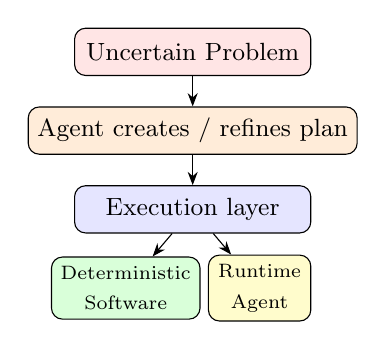
\begin{tikzpicture}[
  box/.style={draw, rounded corners=4pt, minimum width=3.0cm,
              minimum height=0.6cm, align=center, font=\small},
  every node/.style={font=\small}
]
  \node[box, fill=red!10]    (prob) at (0,3.4) {Uncertain Problem};
  \node[box, fill=orange!15] (plan) at (0,2.4) {Agent creates / refines plan};
  \node[box, fill=blue!10]   (exec) at (0,1.4) {Execution layer};
  \node[box, fill=green!15, minimum width=1.3cm] (det) at (-0.85,0.4) {\scriptsize Deterministic\\\scriptsize Software};
  \node[box, fill=yellow!20, minimum width=1.3cm] (rt)  at ( 0.85,0.4) {\scriptsize Runtime\\\scriptsize Agent};
  \draw[-{Stealth}] (prob) -- (plan);
  \draw[-{Stealth}] (plan) -- (exec);
  \draw[-{Stealth}] (exec) -- (det);
  \draw[-{Stealth}] (exec) -- (rt);
\end{tikzpicture}
\end{column}
\end{columns}
% Speaker notes:
% Examples: "I don't know the schema" → agent discovers.
% "I don't know where info lives" → agent searches.
% Sometimes the best use of an agent is to produce deterministic software.
\end{frame}

% ---- Slide 10: Deterministic Code vs Runtime Agent ----
\begin{frame}{Deterministic Code vs.\ Runtime Agent}
After planning, execution can follow different paths:
\vspace{0.4em}
\begin{columns}[T]
\begin{column}{0.48\textwidth}
\begin{block}{Case 1 — Deterministic Execution}
\begin{itemize}
  \item Plan is well specified
  \item Environment is stable
  \item Limited unforeseen events
  \item Output: scripts, workflows, decision trees
\end{itemize}
\end{block}
\end{column}
\begin{column}{0.48\textwidth}
\begin{block}{Case 2 — Runtime Agentic Execution}
\begin{itemize}
  \item Plan remains high-level
  \item Environment is dynamic / non-stationary
  \item System must adapt step by step
  \item Output: ongoing reasoning + actions
\end{itemize}
\end{block}
\end{column}
\end{columns}
\vspace{0.5em}
\begin{center}
\small
\begin{tabular}{lll}
\toprule
\textbf{Dimension}   & \textbf{Deterministic code} & \textbf{Runtime agent} \\
\midrule
Plan specificity     & High              & Medium / Low \\
Environment          & Stable            & Dynamic \\
Adaptation needed    & Low               & High \\
Cost / latency       & Low, predictable  & Higher, variable \\
Debuggability        & Easy              & Harder \\
\bottomrule
\end{tabular}
\end{center}
\vspace{0.3em}
\textit{``Use software where behavior should be fixed. Use runtime agents where behavior must adapt.''}
% Speaker notes:
% Not every problem should stay agentic at runtime.
% Sometimes the best use of an agent is to produce deterministic software.
\end{frame}
  % Anatomy of an Agent
% =======================
% Section 3: Agent Patterns
% =======================
\section{Agent Patterns}

% ---- Slide: ReAct Framework ----
\begin{frame}{ReAct Framework}
\begin{columns}[T]
\begin{column}{0.52\textwidth}
\textbf{ReAct} (Reasoning + Acting)
\begin{itemize}\setlength\itemsep{0.2em}
  \item The canonical single-agent execution pattern
  \item Alternates between:
  \begin{itemize}
    \item \textbf{Thought} --- reason about the next step
    \item \textbf{Act} --- take an action
    \item \textbf{Observe} --- receive result, update beliefs with real-world feedback
    \item \textbf{Repeat} until goal is reached
  \end{itemize}
  \item The \textbf{Observe} step is what a static LLM cannot do - grounding in real-world feedback
\end{itemize}
\end{column}
\begin{column}{0.44\textwidth}
\centering
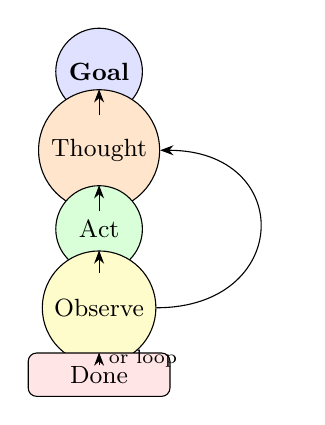
\begin{tikzpicture}[
  node distance=0.7cm,
  stepnode/.style={draw, circle, fill=blue!12, minimum size=1.1cm,
               align=center, font=\small},
  every node/.style={font=\small}
]
  \node[stepnode] (goal)   at (0, 3.2) {\textbf{Goal}};
  \node[stepnode, fill=orange!20] (thought) at (0, 2.2) {Thought};
  \node[stepnode, fill=green!15]  (act)     at (0, 1.2) {Act};
  \node[stepnode, fill=yellow!20] (obs)     at (0, 0.2) {Observe};
  \node[draw, rounded corners=3pt, fill=red!10,
        minimum width=1.8cm, minimum height=0.55cm,
        font=\small] (stop) at (0,-0.65) {Done};

  \draw[-{Stealth}] (goal)   -- (thought);
  \draw[-{Stealth}] (thought) -- (act);
  \draw[-{Stealth}] (act)    -- (obs);
  \draw[-{Stealth}, dashed]  (obs) -- node[right, font=\scriptsize]{or loop} (stop);
  \draw[-{Stealth}] (obs.east) to[out=0,in=0,looseness=2.2] (thought.east);
\end{tikzpicture}
\vspace{0.3em}

\scriptsize Other patterns: \textbf{ReWOO} (plan ahead, no observation loop), \textbf{Reflexion} (self-reflection on errors), \textbf{LATS} (tree search + self-reflection)
\end{column}
\end{columns}
\end{frame}


% ---- Slide: Orchestration Architecture ----
\begin{frame}{Orchestration: Single-Agent vs.\ Multi-Agent}
\begin{columns}[T]
\begin{column}{0.50\textwidth}

\begin{block}{Multi-Agent System}
\begin{itemize}
  \item \textbf{Orchestrator agent}: decomposes the goal, delegates to subagents, synthesizes results
  \item \textbf{Subagents}: specialized, each running its own internal loop
  \item Enables parallelism and role separation
  \item Overhead: coordination, communication, trust between agents
\end{itemize}
\end{block}
\end{column}
\begin{column}{0.46\textwidth}
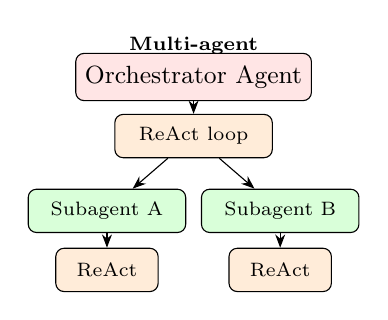
\begin{tikzpicture}[
  box/.style={draw, rounded corners=3pt, minimum width=2.8cm,
              minimum height=0.6cm, align=center, font=\small},
  sbox/.style={draw, rounded corners=3pt, minimum width=2.0cm,
               minimum height=0.55cm, align=center, font=\scriptsize},
  every node/.style={font=\small}
]

  % Multi-agent
  \node[box, fill=red!10] (orch) at (0, 2.3) {Orchestrator Agent};
  \node[sbox, fill=orange!15] (rl0) at (0, 1.55) {ReAct loop};
  \draw[-{Stealth}] (orch) -- (rl0);

  \node[sbox, fill=green!15] (s1) at (-1.1, 0.6) {Subagent A};
  \node[sbox, fill=green!15] (s2) at ( 1.1, 0.6) {Subagent B};
  \draw[-{Stealth}] (rl0) -- (s1);
  \draw[-{Stealth}] (rl0) -- (s2);

  \node[sbox, fill=orange!15, minimum width=1.3cm] (rl2) at (-1.1,-0.15) {\scriptsize ReAct};
  \node[sbox, fill=orange!15, minimum width=1.3cm] (rl3) at ( 1.1,-0.15) {\scriptsize ReAct};
  \draw[-{Stealth}] (s1) -- (rl2);
  \draw[-{Stealth}] (s2) -- (rl3);

  \node[font=\scriptsize\bfseries] at (0, 2.7) {Multi-agent};
\end{tikzpicture}
\end{column}
\end{columns}

\end{frame}

  % Agent Patterns
% =======================
% Section 4: Coding Agents
% =======================
\section{Coding Agents}

% ---- Slide 12: Coding Agents ----
\begin{frame}{Coding Agents and Long-Horizon Autonomous Agents}
\begin{itemize}
  \item \textbf{Why code is a good domain for agents:}
  \begin{itemize}
    \item The environment is structured and well-defined
    \item Tools are explicit: shell, file system, test runner
    \item Success is verifiable — tests pass or fail
    \item Iteration is natural — write, run, observe, fix
  \end{itemize}
  \vspace{0.3em}
  \item Current examples: \textbf{Codex CLI} (OpenAI), \textbf{Claude Code} (Anthropic)
  \item For longer-horizon autonomy: \textbf{OpenClaw} illustrates the direction toward persistent autonomous agents
\end{itemize}
\vspace{0.4em}
\textbf{A spectrum of autonomy:}
\vspace{0.3em}
\begin{center}
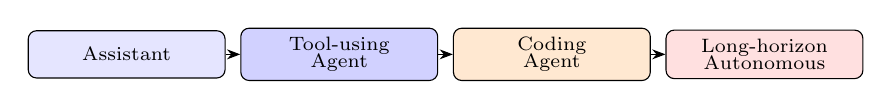
\begin{tikzpicture}[
  box/.style={draw, rounded corners=3pt, fill=blue!10,
              minimum width=2.5cm, minimum height=0.6cm,
              align=center, font=\scriptsize},
  every node/.style={font=\scriptsize}
]
  \node[box]                         (a1) at (0,0)   {Assistant};
  \node[box, fill=blue!18]           (a2) at (2.7,0) {Tool-using\\[-2pt]Agent};
  \node[box, fill=orange!18]         (a3) at (5.4,0) {Coding\\[-2pt]Agent};
  \node[box, fill=red!12, text width=2.2cm] (a4) at (8.1,0) {Long-horizon\\[-2pt]Autonomous};
  \draw[-{Stealth}] (a1) -- (a2);
  \draw[-{Stealth}] (a2) -- (a3);
  \draw[-{Stealth}] (a3) -- (a4);
\end{tikzpicture}
\end{center}
% Speaker notes:
% Verifiability is key: agents work well when "did it work?" has a clear answer.
% That's why code, math, and data pipelines are natural agent domains.
% Reliability, security, and oversight remain major challenges at the long-horizon end.
\end{frame}

% ---- Slide 13: Codex — The Harness and Prompt Assembly ----
\begin{frame}{Codex: The Harness and Prompt Assembly}
\begin{columns}[T]
\begin{column}{0.52\textwidth}
\textbf{Key insight}: Codex separates the \emph{model} from the \emph{harness}
\begin{itemize}
  \item The \textbf{harness} is the orchestration layer that assembles prompts, drives the loop, executes tools, and manages state
  \item ``LLM + tools'' elides exactly this layer — the harness is the agent
\end{itemize}
\vspace{0.3em}
\textbf{Prompt assembly is dynamic} — the prompt the user thinks they send is not what the model sees. The harness assembles it in layers:
\begin{enumerate}
  \item System instructions \textit{(model-specific, bundled in CLI)}
  \item Sandbox / permissions context
  \item Developer instructions
  \item User instructions \textit{(from \texttt{AGENTS.md} files / skills)}
  \item Environment context \textit{(cwd, shell)}
  \item User message
\end{enumerate}
\vspace{0.2em}
\small Native tools, Responses API tools, and MCP tools all appear \emph{identical} to the model in the tools array.
\end{column}
\begin{column}{0.44\textwidth}
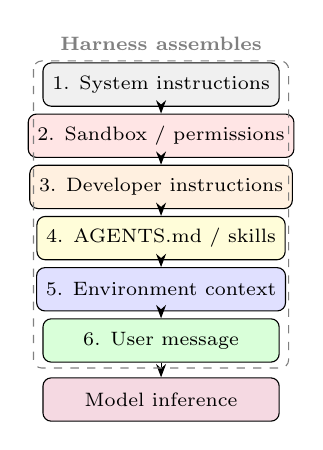
\begin{tikzpicture}[
  box/.style={draw, rounded corners=3pt, fill=blue!10,
              minimum width=3.0cm, minimum height=0.55cm,
              align=center, font=\scriptsize},
  every node/.style={font=\scriptsize}
]
  \node[box, fill=gray!12]   (sys)  at (0, 4.2) {1. System instructions};
  \node[box, fill=red!10]    (sand) at (0, 3.55) {2. Sandbox / permissions};
  \node[box, fill=orange!12] (dev)  at (0, 2.9) {3. Developer instructions};
  \node[box, fill=yellow!15] (agmd) at (0, 2.25) {4. AGENTS.md / skills};
  \node[box, fill=blue!12]   (env)  at (0, 1.6) {5. Environment context};
  \node[box, fill=green!15]  (usr)  at (0, 0.95) {6. User message};
  \node[box, fill=purple!15] (inf)  at (0, 0.2) {Model inference};

  \draw[-{Stealth}] (sys)  -- (sand);
  \draw[-{Stealth}] (sand) -- (dev);
  \draw[-{Stealth}] (dev)  -- (agmd);
  \draw[-{Stealth}] (agmd) -- (env);
  \draw[-{Stealth}] (env)  -- (usr);
  \draw[-{Stealth}] (usr)  -- (inf);

  \draw[dashed, gray, rounded corners=3pt]
    (-1.62, 4.5) rectangle (1.62, 0.6);
  \node[font=\scriptsize\bfseries, text=gray] at (0, 4.72) {Harness assembles};
\end{tikzpicture}
\end{column}
\end{columns}
% Speaker notes:
% Connect to Slide 2 (Anatomy): the harness IS the control + action + state layers made concrete.
% Skills appear here as AGENTS.md / skill files — this is the Codex instantiation of the concept.
% MCP safety reminder: MCP tools are NOT sandboxed by Codex.
\end{frame}

% ---- Slide 14: Codex — Managing the Growing Context ----
\begin{frame}{Codex: Managing the Growing Context}
\begin{columns}[T]
\begin{column}{0.52\textwidth}
\textbf{The prompt grows monotonically:}
\begin{itemize}
  \item Each turn appends to prior input — full conversation history always included
  \item A single turn can contain many iterations of inference + tool calls
  \item A turn ends only when the model emits an \emph{assistant message} (termination signal)
  \item This is \textbf{quadratic} in data sent — a real engineering problem
\end{itemize}
\vspace{0.3em}
\textbf{Two mitigations:}
\begin{itemize}
  \item \textbf{Prompt caching} — reuse computation from prior inference if the prefix is stable. Static content (instructions, tools) must come first; variable content last. \textit{Cache miss}: MCP tools enumerated in inconsistent order $\to$ expensive miss every turn.
  \item \textbf{Automatic compaction} — when token threshold exceeded, conversation is summarized and replaced with a compressed representation, preserving the model's latent understanding via encrypted content
\end{itemize}
\end{column}
\begin{column}{0.44\textwidth}
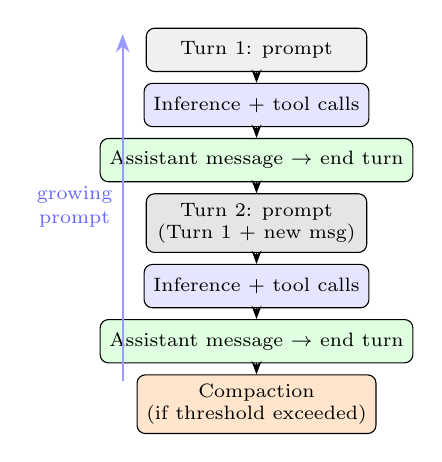
\begin{tikzpicture}[
  box/.style={draw, rounded corners=3pt, fill=blue!10,
              minimum width=2.8cm, minimum height=0.55cm,
              align=center, font=\scriptsize},
  every node/.style={font=\scriptsize}
]
  \node[box, fill=gray!12]   (t1) at (0, 4.2) {Turn 1: prompt};
  \node[box, fill=blue!10]   (i1) at (0, 3.5) {Inference + tool calls};
  \node[box, fill=green!12]  (a1) at (0, 2.8) {Assistant message $\to$ end turn};

  \node[box, fill=gray!20]   (t2) at (0, 2.0) {Turn 2: prompt\\(Turn 1 + new msg)};
  \node[box, fill=blue!10]   (i2) at (0, 1.2) {Inference + tool calls};
  \node[box, fill=green!12]  (a2) at (0, 0.5) {Assistant message $\to$ end turn};

  \node[box, fill=orange!20] (cp) at (0,-0.3) {Compaction\\(if threshold exceeded)};

  \draw[-{Stealth}] (t1) -- (i1);
  \draw[-{Stealth}] (i1) -- (a1);
  \draw[-{Stealth}] (a1) -- (t2);
  \draw[-{Stealth}] (t2) -- (i2);
  \draw[-{Stealth}] (i2) -- (a2);
  \draw[-{Stealth}, dashed] (a2) -- (cp);

  % Growing arrow
  \draw[{Stealth}-, thick, blue!40] (-1.7, 4.4) -- (-1.7, -0.0)
    node[midway, left, font=\scriptsize, blue!60] {\shortstack{growing\\prompt}};
\end{tikzpicture}
\end{column}
\end{columns}
% Speaker notes:
% Connect to Appendix B failure mode "excessive cost / latency" — now students see the mechanism.
% The MCP tool reordering bug is a perfect real example of how implementation details
% have direct cost impact in production.
% Key lesson: the agent loop is not just about reasoning — it is about context budget management.
\end{frame}
  % When to Use Agentic AI
% =======================
% Section 5: Demo
% =======================
\section{Demo}

% ---- Slide 15: Transition to the Notebook Demo ----
\begin{frame}{Transition to the Notebook Demo}
\begin{columns}[T]
\begin{column}{0.52\textwidth}
\textbf{Next:} build a simple agent in AWS\\[0.6em]
Goals of the demo:
\begin{itemize}
  \item Define tools (and expose via MCP)
  \item Configure the model
  \item Create the agent
  \item Interact with it
\end{itemize}
\vspace{0.6em}
Focus: making the abstractions \textbf{concrete}\\[0.4em]
\textit{``Now that we have the conceptual map, we move to a practical implementation.''}
\end{column}
\begin{column}{0.44\textwidth}
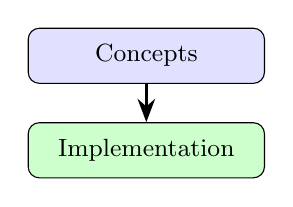
\begin{tikzpicture}[
  box/.style={draw, rounded corners=4pt, minimum width=3.0cm,
              minimum height=0.7cm, align=center, font=\small},
  every node/.style={font=\small}
]
  \node[box, fill=blue!12]  (concept) at (0,1.6) {Concepts};
  \node[box, fill=green!20] (impl)    at (0,0.4) {Implementation};
  \draw[-{Stealth}, very thick] (concept) -- (impl);
\end{tikzpicture}
\end{column}
\end{columns}
% Speaker notes:
% The notebook is intentionally simpler than the full theory stack.
% Not every production concern will be implemented live,
% but students will see the essential agent loop.
\end{frame}

% =======================
% Appendix
% =======================
\appendix

\begin{frame}{Appendix A — Memory Types}
\begin{itemize}
  \item \textbf{Working / context memory} — current prompt and conversation window; ephemeral
  \item \textbf{Short-term / session memory} — state maintained across turns within a session
  \item \textbf{Long-term / persistent memory} — durable storage across sessions (external store)
\end{itemize}
\vspace{0.4em}
\small \textit{Memory captures what the agent experienced. The knowledge base captures what exists in the domain. Both feed into the context window at inference time — they are complementary, not alternatives.}
\end{frame}

\begin{frame}{Appendix B — Failure Modes of Agents}
\begin{itemize}
  \item \textbf{Hallucination} — confident but incorrect outputs
  \item \textbf{Wrong tool selection} — choosing an inappropriate tool for a task
  \item \textbf{Looping} — repeating the same steps without progress
  \item \textbf{Stale retrieval} — outdated or irrelevant chunks returned by RAG
  \item \textbf{Prompt injection} — malicious instructions embedded in retrieved content or tool outputs hijack the agent
  \item \textbf{Permission leakage} — agent accesses data or tools beyond its authorization
  \item \textbf{Excessive cost / latency} — runaway token usage or slow chains; the growing context window is a key structural driver
\end{itemize}
\end{frame}

\begin{frame}{Appendix C — Alternative Agent Execution Patterns}
\begin{itemize}
  \item \textbf{ReAct} — Thought $\to$ Act $\to$ Observe loop; grounded in real-world feedback at each step
  \item \textbf{ReWOO} — plans all tool calls upfront without an observation loop; more efficient but less adaptive
  \item \textbf{Reflexion} — adds iterative self-reflection; agent identifies errors and revises strategy
  \item \textbf{LATS} (Language Agent Tree Search) — builds a decision tree over possible actions using Monte Carlo search + self-reflection; excels at complex coding and QA tasks
\end{itemize}
\vspace{0.4em}
\small All of these are single-agent execution patterns. They operate at a different level from orchestration architecture (single-agent vs.\ multi-agent system design).
\end{frame}
  % End-to-End Example
% =======================
% Section 6: Notebook
% =======================
\section{Lab}

% ---- Slide 15: Transition to the Notebook Demo ----
\begin{frame}[t]{Lab}

\textbf{Lab: Building an Agentic AI Chatbot}\\[0.3em]
\small From theory to practice: putting the agent loop, tools, and memory to work.\\[0.3em]
\footnotesize \url{https://github.com/awslabs/agentcore-samples/blob/main/01-tutorials/09-AgentCore-E2E/strands-agents/lab-01-create-an-agent.ipynb}

\centering
\vspace{0.5em}
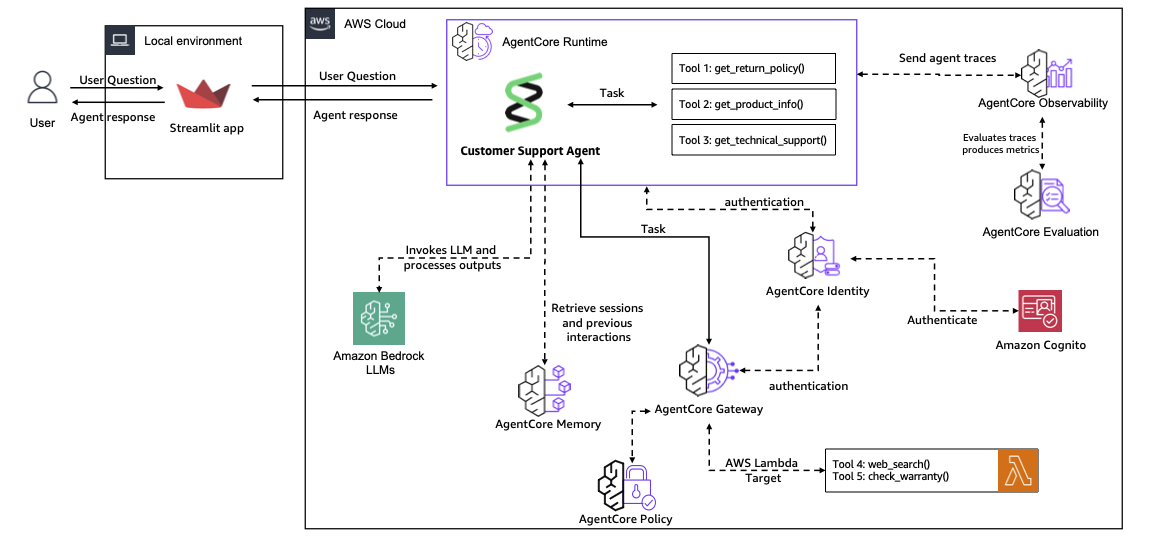
\includegraphics[width=1\textwidth]{images/architecture_lab6_streamlit.png}

% Speaker notes:
% The notebook is intentionally simpler than the full theory stack.
% Not every production concern will be implemented live,
% but students will see the essential agent loop.
\end{frame}
  % Notebook

\end{document}
